

\section{The Digital Image}
\greenbf{Problems:} Transmission interference, compression artifacts, spilling, scratches, sensor noise, bad contrast and resolution, motion blur \\
\greenbf{Pixel:} Discrete samples of an continuous image function.\\
\greenbf{Rolling Shutter} effect produced by sequential readout of pixels while a digital camera is moving. Result is pixels read at different times are sequentially misaligned, causing image-level distortions dependent on camera (or object) movement.
\subsection*{Charge Coupled Device \graytext{(CCD)}}
Has an array of photosites \graytext{(a bucket of electrical charge)} that charge proportional to the incident light intensity during exposure. ADC happens line by line. \\
\greenbf{Bloooming:} oversaturation of finite capacity photosites causes the vertical channels to "flood" \graytext{(bright vertical line)}\\
\greenbf{Bleeding/Smearing:} While shifting down, the pixels above get some photons on bright spot with electronic shutters.\\
\greenbf{Dark Current:} CCDs produce thermally generated charge they give non-zero output even in darkness \graytext{(fluctuates randomly)} due to spontaneous generation of electrons due to heat $\rightarrow$ cooling.\\ can be avoided by cooling, worse with age.
\subsection*{CMOS:}
Same sensor elements as CCD, but each sensor has its own amplifier $\rightarrow$ faster readout, less power consumption, cheaper, more noise.\\ more noise, lower sensitivity\\
\greenbf{vs CCD} cheaper, lower power, less sensitive, per pixel amplification random pixel access, no blooming, on chip integration

\begin{tabularx}{\linewidth}{|X|X|X|X|}
    \hline
    Approach & Prism & Mosaic & Wheel \\ \hline
    \# Sensors & 3 & 1 & 1 \\ \hline
    Separation & High & Avg. & Good \\ \hline
    Cost & High & Low & Average \\ \hline
    Framerate & High & High & Low \\ \hline
    Artifacts & Low & Aliasing & Motion \\ \hline
    Bands & 3 & 3 & \(\geq 3\) \\ \hline
    Usage & High-End & Low-end & Scientific \\ \hline
  \end{tabularx}

\subsection*{Sampling methods}
Cartesian \graytext{(grid)}, hexagonal, non-uniform\\
\greenbf{Quantization:} Real valued function will get digital values \graytext{(integers)}. A lossy process \graytext{(original cannot be reconstructed)}. Simple version: equally spaced $2^b = \#bits$ levels\\
\greenbf{Linear Interpolation}: \\
$p(t) = p_0 + (t - t_0)\frac{p_1 - p_0}{t_1 - t_0} \text{ with } t \in [t_0, t_1]$ \\

\greenbf{Bilinear Interpolation:}     \\
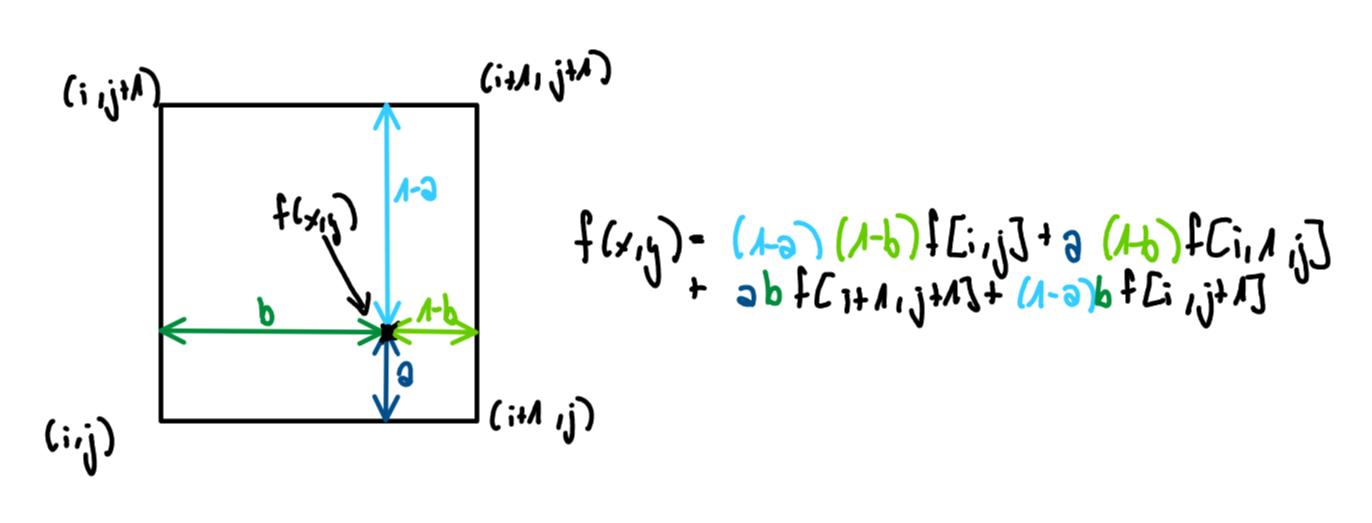
\includegraphics[width=\columnwidth]{jo/linear-interpolation.png} \\ 
\greenbf{Resolution}
    \begin{compactitem}
      \item \textit{Image}: px \(\times\) px
      \item \textit{Geometric}: \#pixels per area
      \item \textit{Radiometric}: \#bits per pixel
    \end{compactitem}
\greenbf{Image noise:} commonly modeled by additive Gaussian noise: $I(x, y) = f(x, y) + c$, poisson noise \graytext{(shot noise for low light, depends on signal \& aperture time)}, multiplicative noise: $I = f + f \cdot c$, quantization errors, salt-and-pepper noise. SNR or peak SNR is used as an index of image quality $c \sim N(0, \sigma^2)$, $p(c) = \frac{1}{\sigma \sqrt{2\pi}} \cdot \exp\left(-\frac{(c - \mu)^2}{2\sigma^2}\right)$, SNR: $S = \frac{F}{\sigma}$ where $F = \frac{1}{XY}\sum_{x = 1}^X \sum_{y = 1}^{Y} f(x, y)$.
\subsection*{Color cameras}
\greenbf{Prism} need 3 sensors and good alignment\\
\greenbf{Filter mosaic} coat $\square$ directly on sensor \\
\greenbf{Wheel} multiple filters in front of same sensor\\
\greenbf{New CMOS sensor} layers that absorb color at different depths $\rightarrow$ better quality